\documentclass[]{article}
\usepackage[utf8]{inputenc}
\usepackage[T1]{fontenc}
\usepackage[english]{babel}
\usepackage[top=2cm, bottom=3cm, left=3cm, right=3cm]{geometry}
\usepackage{amsmath}
\usepackage{graphicx}
\graphicspath{{figure/}}
\usepackage{hyperref}

% Rq: To display code like text, just use \begin{verbatim} or \verb#blabla#
\newcommand{\sepline}{\begin{center}\rule{0.5\linewidth}{\linethickness}\end{center}}

\title{A simple example: the lactose operon}
\author{P. \textsc{François}, M. \textsc{Hemery}, A. \textsc{Henry}}

\begin{document}

\maketitle{}

\section{Description of the biological
problem}\label{description-of-the-biological-problem}

The lactose operon is one of the most studied example in the regulation of
proteins production. In \textit{Escherichia coli}, the operon\footnote{
In genetics, an operon is a functioning unit of DNA, it designates
a cluster of genes under the control of a single promoter.} encodes three
different genes named lacZ, lacY and lacA from which the two firsts are
the most importants. LacZ codes for a protein that hydrolizes lactose
to produce glucose and galactose, which are themselves used by the cell as
carbon sources. LacY encodes a permease, a protein which pumps the
lactose into the cell. Both of these proteins need to be
synthesized by the cell to use the lactose as an energy source, but as this
is costly, and less efficient than using the glucose directly, the cell
manages to produce them only in presence of lactose and in absence of
glucose.

\begin{figure}
\centering
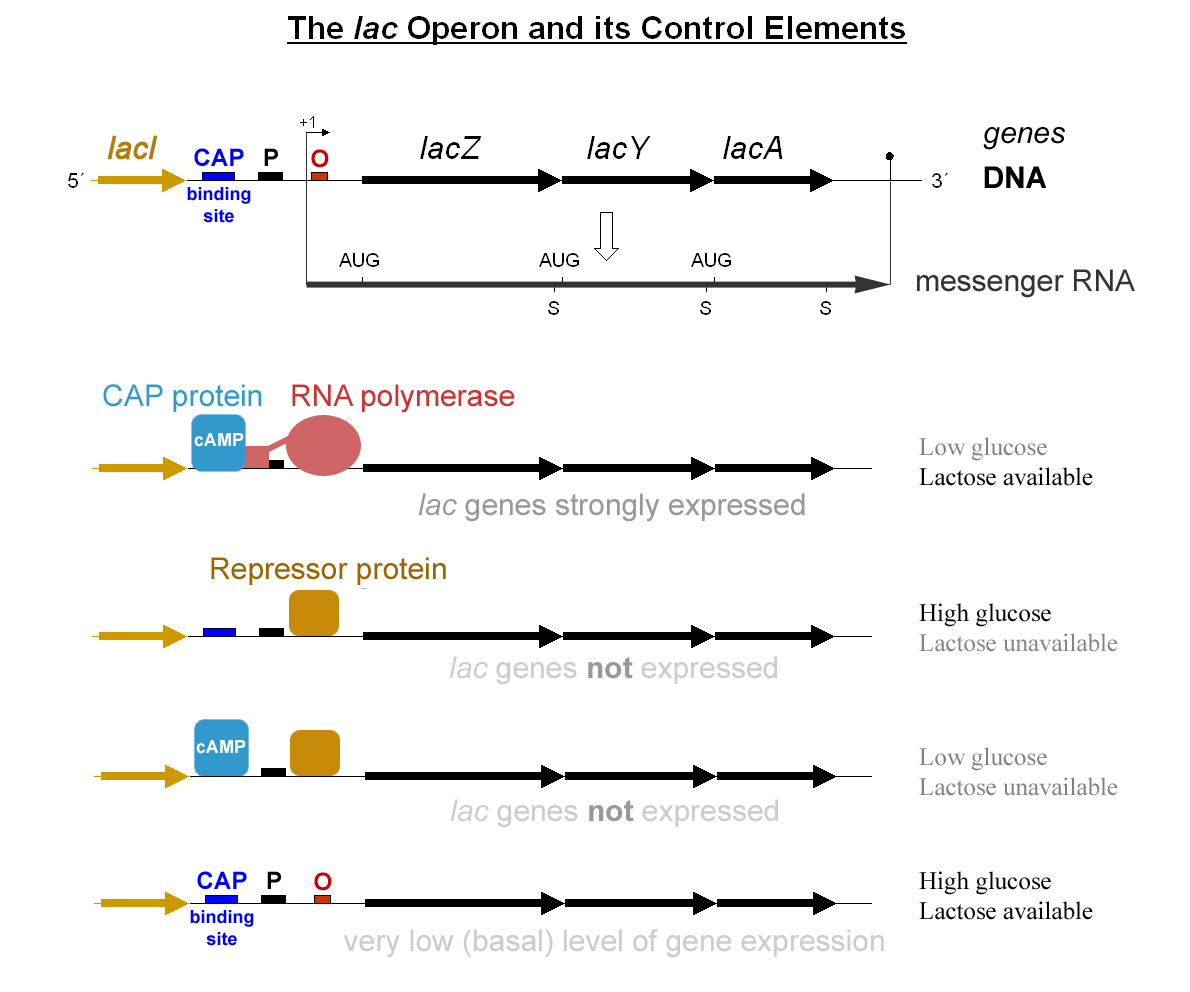
\includegraphics[width=.6\textwidth]{lac_operon_presentation}
\caption{Scheme presenting the main elements of the lactose operon along 
the DNA strain (top), and the state of the operon through several external 
conditions (bottom). Published on
\href{https://commons.wikimedia.org/wiki/File:Lac_operon-2010-21-01.png}{Wikimedia}
by G3pro and Tereseik.}
\label{fig:lac_operon}
\end{figure}

Cells have thus designed a logical gate, schematically shown in
figure~\ref{fig:lac_operon}, to compute the binary function:
\emph{lactose and no glucose} that controls the expression of the whole operon.
The biological strategy is the following: near the operon, the gene lacI
encodes a repressor of the operon which is constitutively expressed so
that by default, the operon is turned off. When lactose is present in
the medium, a closed form, the allolactose is also present and will bind
to the lacI repressor, thus impeding it to block the operon. It is now
possible to expressed the operon but there is still no activation. The
activator, the CAP protein, is indeed in an active form only in the
presence of cAMP which is produced in absence of glucose\footnote{For curious
reader, the reason why, when energy tends to rarify, the cell suddenly produces
an extraodinary amount of seemingly useless proteins is still an active 
question!}. As long as
glucose is present, the operon is still silent and it is only when
glucose become rare that cAMP goes high, thus activating the CAP protein
which activate the operon and thus the production of the needed
proteins.

Hereafter, we will run our genetic algorithm to optimize a function close
from the logical gate corresponding to the lac operon, that is: $x,y \mapsto 
x~\&~\neg y$, the link with the biology of the real lac operon would
nonetheless ask more work than will be presented here.

\section{Implementation in the
algorithm}\label{implementation-in-the-algorithm}

\paragraph{Remark}
All files, functions and variables names along with terminal commands will
be printed using the \LaTeX{} environment verbatim and display
with \verb#this particular font#.

\vspace{1em}

Two mains questions need to be answered in order to configure the
algorithm for a particular problem. What? and How?~: What is the
precise function we need to optimize in order to describe the problem?
and How the solution is allowed to be found by the algorithm? The first
will be mainly described by the C code files like \verb#init_history.c# and
\verb#fitness.c# while the second will be solved through the tuning of the
various parameters in the so called \verb#init*.py# file.

\sepline{}

The \verb#init_history.c# file describes the form of the input(s) that
will be feed into the network. This is done through the construction of
the double array \verb#isignal[time][n_cell][n_input]# which indicates 
the concentration of the various input with respect to the time and cell.

In our case, we have two inputs that will
represent the concentration of glucose and lactose and will be taken as
binary functions (each sugar has a concentration of $0.0$ or $1.0$) which follow
a random sequence of presence and absence, the time being spent in each state 
uniformly drawn between \(10\) and \(60\) seconds (see figure~\ref{fig:response_lo}).

\vspace{1em}

The \verb#fitness.c# file intend to process the output of the
integrator which is rounded up in the double array named history indexed in the
following way: \verb#history[Species][Time][Cell]#. The variables
\verb#trackin# and \verb#trackout# keeps in memory the label of the inputs and
outputs species. The fitness is directly printed out by the \verb#treatment_fitness#
function. (Note however, that \verb#treatment_fitness# is a void,
fitness is passed with the \verb#printf("%f",fitness);# statement.)

For lac operon simulation, each try of the integrator is treated
independantly and follow the time course of the input and output to
determine the times at which production is needed (that is when there is
lactose and no glucose) and the concentration of the output at that
time. We then have chosen to compute the mutual information\footnote{
The mutual information of two random variables is a way to quantify the
information I can extract about one variable by measuring the second.}
between $\text{lactose}~\&~\neg \text{glucose}$ and the concentration
of the output.

\vspace{1em}

Finally, the \verb#init*.py# file indicate the mutation rates of the
different interactions, the number of networks in the population, the
number of generation of the simulation, the initial
network from which we want to start and so on.

In the case of the
lac\_operon, we will ask the algorithm to use only protein-protein
interaction (PPI) and repression/activation of gene (TFHill) and put
to zero the parameters indicating the appearance of other interactions,
for example:
\begin{verbatim}
    random_Interaction('Degradation') = 0
    random_Interaction('Phosphorylation') = 0
\end{verbatim}
which control the rate at which
new degradations and phosphorylations are added to the network to be
probed by the evolution.

\sepline{}

Each of this file has to be put in a single folder (in our case
\verb#lac_operon/#) in order to be found by the algorithm. Evolutionary
procedure is now simply launched by running the
\begin{verbatim}
    python run_evolution.py -m lac_operon
\end{verbatim}
command line while in the main
folder. The algorithm will now display a lot of more or less important
stuff in your terminal. The most interesting are the generation number
which indicate at which point of your simulation you are. When
accustomed to it, the \verb#Best_fitness# is an interesting variable to look
at to know if the condition you defined actually allow the algorithm to
find valid solution for the problem. Finally, every line starting
by \verb#ERROR# needs of course your special attention.

\begin{figure}
\centering
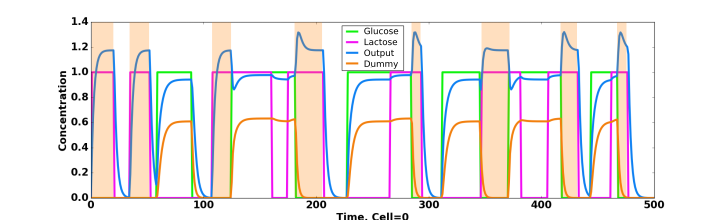
\includegraphics[width=.8\textwidth]{p2_response}
\caption{Detailed response of the network presented in
fig~\ref{fig:network_lo}{\bf A}, colors correspond between the two figures.
Orange shades indicate the time at which response is waited.}
\label{fig:response_lo}
\end{figure}

\subsection*{A word about fitness}\label{a-word-about-fitness}

In order for the evolutionary procedure to give meaningful results, a
special attention need to be given to design a proper fitness function.
There is several reasons for this particular importance but the main one
is that the algorithm will only try to solve the exact problem you have
defined -- i.e. minimize the fitness function you have provided -- which
is usually different from the actual task you have in mind.

For example, one of the solution proposed by the algorithm for the
lac\_operon fitness proposed earlier (the mutual information between the
output concentration and the $\text{lactose}~\&~\neg \text{glucose}$ function) was to use
lactose as a weak activator of the output and glucose as\ldots{} a
strong activator of the output! When looking at the time
course of the output concentration, it makes plain sense because the
concentration is near zero when there is no sugar, goes to one when
there is only lactose and saturate around two when there is either
glucose only or when both sugare are presents. Thus if the concentration
is around one you know that you have lactose and no glucose. You can
extract the whole information about the $\text{lactose}~\&~\neg \text{glucose}$
function from the output concentration which is the
task we ask for, even if the answer was quite surprising.

This also mean that you will often want to modify your fitness function after
a first bunch of runs to be more explicit or to try a different fitness function.
To avoid being rapidly lost between your different simulation, you can
look at the \verb#Seed*/log_fitness.c# file for a reminder of the fitness
used at this time.

A second remark about fitness is that the function should goes smoothly
from the low fitness landscape to the region you want to explore, that
is the fitness function should already rewards the first steps toward the
solution. Otherwise, the algorithm will be stuck in the low level region
and cannot even start to optimize. This question covers a broad range of
litterature both in evolutionary biology and genetic algorithm computer
science around the fitness-landscape shape question with suggestive
names such as mount Fuji, house of cards or golf-course. It is usually
not a big deal but could bring you some surprise if you don't keep it in
mind.

\section{How to read and interpret
results}\label{how-to-read-and-interpret-results}

Now that your computer has run several simulations it is time to analyse
them to decipher the output of the evolutionary algorithm. The first
thing to look at is the time course of the fitness for several runs, to
show the fitness of the first run, you can either use the \verb#Analyse run#
notebook or type in your terminal.
\begin{verbatim}
    python analyse_run.py lac_operon 0
\end{verbatim}
Make sure to check several runs to know the typical fitness of
a successful or failed run, this will discard the cases where the evolutionary
algorithm has been stuck and doesn't have enough time to converge.

To study a particular network, you can now type \verb#network(500)# if you
want to display the state of the best network in the population at
generation $500$ (the end of the simulation given our \verb#init*.py# files).
It may be small and concise but usually it's not, evolutionary procedure
tends to accumulate a lot of uninteresting interactions and species -- the
famous DNA junk? --that mey be ignored.
Anyway, this is the raw result of the evolution. To save a particular
network, just type \verb#save(500)#. It will print out the file
directory where the network has been saved for later analysis.

\vspace{1em}

You can now turn to the \verb#analyse_network# module by invoking it from the
terminal and providing the model you are studying.
\begin{verbatim}
    python analyse_network.py -m lac_operon
\end{verbatim}
You can from there read and write
network (with the read and write function), compute the fitness (with
the \verb#fitness# function) and even look at the time course of the species
for a particular realisation of the fitness computation. If net is your
network, just type \verb#fitness(net, plot=True)#. You can also plot a
network using \verb#net.draw()#.

Finally, you can also add homebrew function to analyse your evolutionary
result by adding a \verb#analyse.py# file in the project folder. It will
be imported with \verb#analyse_network# through the name \verb#spec#.

\begin{center}\rule{0.5\linewidth}{\linethickness}\end{center}

To make your final network more insightful, you may want to prune your
network by removing the less usefull interactions. Several functions of
the \verb#analyse_network.py# module are useful for this task:

\begin{itemize}
\item
  \verb#clone(net)#: Return a deepcopy of the network, use it to save
  your network before making a critical move.
\item
  \verb#net.draw(edgeLegend=True)#: plot the network in a pyplot frame.
  The \verb#edgeLegend# option add more information about interactions
  to simplify the reading and pruning procedure but is off by default for
  aesthetics.
\item
  \verb#fitness(net,plot=False)#: Compute the fitness as it is done by
  the algorithm, if plot is set to \emph{True}, it also display the time
  course of the different species in the network as a function of time
  for a particular try (the first one by default). It can be use to
  manually check that your modification doesn't alter the fitness in a
  harmfull way.
\item
  \verb#pruning(net)#: An automatic function which try to set all the
  parameters of the network to zero or ten one after the other and then
  remove the interactions which obviously seems useless. This can
  however missed several parts of the network, so a manual pruning is
  usually needed after this first round.
\item
  \verb#read(filename)#/\verb#write(net,filename)#: allow you to fetch and
  store networks (try to keep the \verb#.net# extension). The project
  folder path is automatically added.
\item
  \verb#remove_interaction(net,id)#: Delete the interaction of the
  network whom label is \verb#n[id]#. You shouldn't remove species
  directly, instead, call \verb#remove_interaction# on the one which create
  the species (CorePromoter for a free Species for example).
\end{itemize}

\begin{center}\rule{0.5\linewidth}{\linethickness}\end{center}

\begin{figure}
\centering
{\bf A.}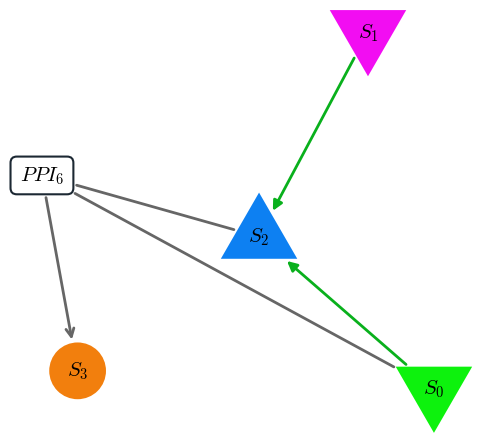
\includegraphics[width=.3\textwidth]{p2_network}
~~~~
{\bf B.}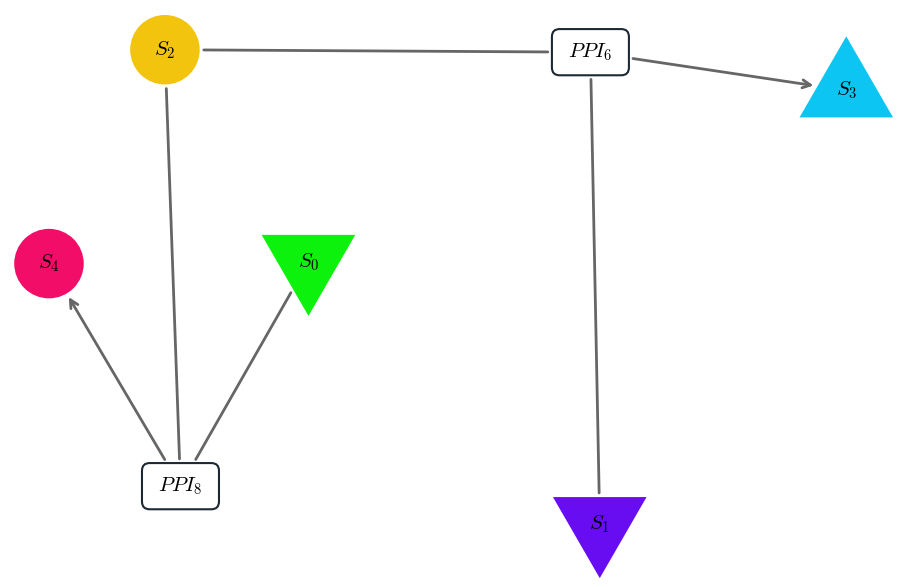
\includegraphics[width=.4\textwidth]{p31_network}
\caption{Pannels {\bf A.} and {\bf B.} shows two typical topologies of the final result
of the algorithm trying to optimize our mutual-information fitness. In both pannel,
inputs are species $0$ (glucose) and $1$ (lactose) (down-triangle) and output is the up-triangle.
{\bf A.} Both sugars regulate positively the output, but the glucose also form a
dimer with it thus impeding the response. The time course of this network is
displayed in fig~\ref{fig:response_lo}.
{\bf B.} Here a single species (S2) can form two complexes, one very strongly with
the glucose (S4), and another weaker with the lactose (S3). The former complex being the
output.}
\label{fig:network_lo}
\end{figure}

In our case, out of 10 runs, 80\% ended on 2 main different topologies (after
pruning) both performing correctly, that is the fitness plateau around 
$-0.8$ on a scale of $0$ to $-1$. Four correspond to the network of
figure~\ref{fig:network_lo}{\bf A} while four other looks like the one in
figure~\ref{fig:network_lo}{\bf B}. I let up to you the biological
interpretation of these results\footnote{Just a hint, for case {\bf B} 
it seems to me that species 2 should be considered as the DNA strain!}
but the first obvious feature is the uniformity of the solution. Nearly
all the successfull runs show very similar patern indicating that the
biological grammar available actually imposes strong constraints on the
possibles solution to a particular problem.

\section{and Beyond}\label{and-beyond}

To take advantage of the other options of the algorithm, we will give
here a brief presentation of its additional features:

\paragraph{Pareto Evolution}\label{pareto-evolution}

The notion of Pareto optimality came from the economy and intend to
evaluate a list of objects along several criteria when no obvious
trade-of or hierarchy can be made among the different criteria. Pareto
optimality class objects which are better along every criterion as
better but consider equal objects which are better only along some of
them\footnote{As a particular example, suppose you want to buy a chair.
You want it comfy, robust and cheap, if you can have more comfort
without decreasing robustness nor increasin price… that's better,
but between the cheap one and the costly but better, it is ultimately
a matter of taste.}.

Our evolution implement a Pareto ranking algorithm that can be activated
in the \verb#init*.py# file. It ask you the number of criteria you wan't to
take into account. This criteria should be printed by the \verb#fitness.c# file
one number per line.

However, you may notice that several concepts break when pareto
evolution is used. Particularly, the notion of best individual is quite
fuzzy and the mean fitness of the population doesn't have much sense.
The function \verb#analyse_run.pareto_scatter# allow you to investigate
the repartition of the population in the fitness space (when there is 2
or 3 fitness criteria).

\paragraph{Geometry}\label{geometry}

\paragraph{New interactions}\label{new-interactions}

\end{document}
